\documentclass[tikz]{standalone}
\usepackage{amsmath}
\definecolor{bgdark}{HTML}{171D2B}
\definecolor{aksen}{HTML}{F7B538}
\newcommand{\lbl}[1]{{\color{black}#1}}
\begin{document}
\pagecolor{bgdark}
\color{white}
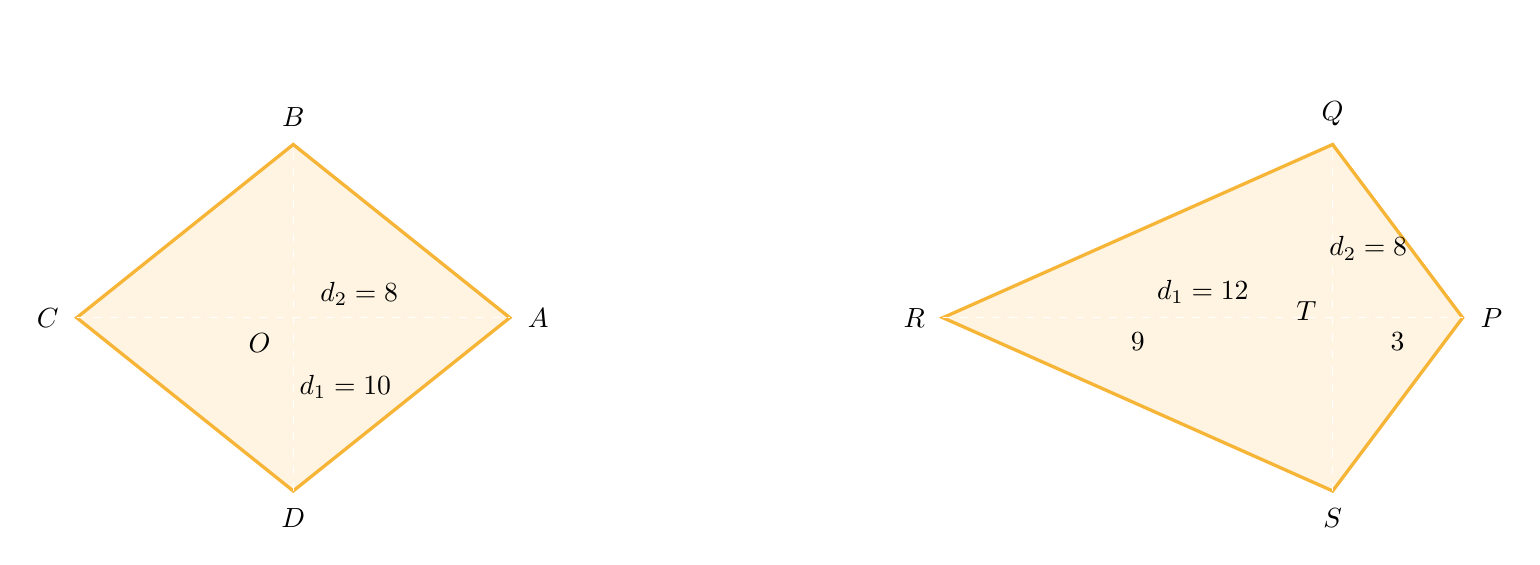
\begin{tikzpicture}[scale=0.55]
  % ===== Belah ketupat: diagonal d1=10, d2=8 =====
  \begin{scope}[xshift=-9cm]
    \coordinate (A) at ( 5, 0);
    \coordinate (B) at ( 0, 4);
    \coordinate (C) at (-5, 0);
    \coordinate (D) at ( 0,-4);
    \coordinate (O) at ( 0, 0);
    \draw[very thick, aksen, fill=aksen!15] (A) -- (B) -- (C) -- (D) -- cycle;
    \draw[dashed, white] (C) -- (A);
    \draw[dashed, white] (D) -- (B);
    \node[black] at (1.2,-1.6) {\lbl{$d_1 = 10$}};
    \node[black, anchor=west] at (0.4,0.55) {\lbl{$d_2 = 8$}};
    \node[black, anchor=north east] at (-0.3,-0.15) {\lbl{$O$}};
    \node[right=3pt] at (A) {$A$};
    \node[above=3pt] at (B) {$B$};
    \node[left=3pt]  at (C) {$C$};
    \node[below=3pt] at (D) {$D$};
    \node[white] at (0,6.2) {\textbf{Belah Ketupat}};
  \end{scope}
  % ===== Layang-layang: d1=12, d2=8, potong di 3:9 =====
  \begin{scope}[xshift=9cm]
    \coordinate (P) at ( 9, 0);
    \coordinate (Q) at ( 6, 4);
    \coordinate (R) at (-3, 0);
    \coordinate (S) at ( 6,-4);
    \coordinate (T) at ( 6, 0);
    \draw[very thick, aksen, fill=aksen!15] (P) -- (Q) -- (R) -- (S) -- cycle;
    \draw[dashed, white] (R) -- (P);
    \draw[dashed, white] (S) -- (Q);
    \node[black] at (3,0.6) {\lbl{$d_1 = 12$}};
    \node[black, anchor=west] at (5.7,1.6) {\lbl{$d_2 = 8$}};
    \node[black] at (1.5,-0.55) {\lbl{$9$}};
    \node[black] at (7.5,-0.55) {\lbl{$3$}};
    \node[black, anchor=south east] at (5.85,-0.3) {\lbl{$T$}};
    \node[right=3pt] at (P) {$P$};
    \node[above=3pt] at (Q) {$Q$};
    \node[left=3pt]  at (R) {$R$};
    \node[below=3pt] at (S) {$S$};
    \node[white] at (3,6.2) {\textbf{Layang-Layang}};
  \end{scope}
\end{tikzpicture}
\end{document}
